%!TEX root=paper.tex
\section{Gilbert Runtime}
\label{sec:gilbertRuntime}

The Gilbert runtime is responsible for executing the compiled MATLAB code on a particular platform. 
For this purpose, it receives the intermediate representation of the code and translates it into the execution engine's specific format. 
Currently, Gilbert supports three different execution engines: \emph{ReferenceExecutor}, \emph{FlinkExecutor} and \emph{SparkExecutor}. 
The \emph{ReferenceExecutor} executes the compiled MATLAB code locally. 
For the distributed execution Gilbert supports Apache Spark and Apache Flink as backends. 

The \emph{ReferenceExecutor} is an interpreter for the intermediate code.
It takes the dependency tree of a MATLAB program and executes it by evaluating the operators bottom-up. 
In order to evaluate an operator, the system first evaluates all inputs of an operator and then executes the actual operator logic. 
Since the program is executed locally, the complete data of each operator is always accessible and, thus, no communication logic is required. 
All input and output files are directly written to the local hard drive. 

In contrast to the \emph{ReferenceExecutor}, the \emph{FlinkExecutor} and \emph{SparkExecutor} execute the program in parallel. 
Consequently, data structures are needed which can be distributed across several nodes and represent the commonly used linear algebra abstractions, such as vectors and matrices. 
Moreover, the linear algebra operations have to be adjusted so that they keep working in a distributed environment. 
Since both systems offer a similar set of programming primitives, they can operate on the same data structures. 
Furthermore, most of the linear algebra operations are implemented in a similar fashion.
The details of the distributed data structures and operations are explained in \cref{sec:DistributedMatrixRepresentation} and \cref{sec:LinearAlgebraOperations}.

\subsection{Distributed Matrix Representation}
\label{sec:DistributedMatrixRepresentation}

An important aspect of distributed algorithms is how their data is distributed. 
Since the distribution pattern directly influences the algorithms, one cannot consider them independently from one another. 
In Gilbert's use case, the main data structure are matrices. 
Thus, the matrix entries have to be partitioned.
A first idea could be to partition a matrix according to their rows or columns, as it is depicted in \cref{fig:rowPartitioning} and \cref{fig:columnPartitioning}. 
This scheme allows to represent a matrix as a distributed set of vectors.
Furthermore, it allows an efficient realization of cellwise operations, such as $+,-,/$ or $.*$. 
In order to calculate the result of such an operation, we only have to join the corresponding rows of both operands and execute the operation locally for each pair of rows.

\begin{figure}[htbp]
	\centering
	\begin{subfigure}{.3\linewidth}
		\centering
		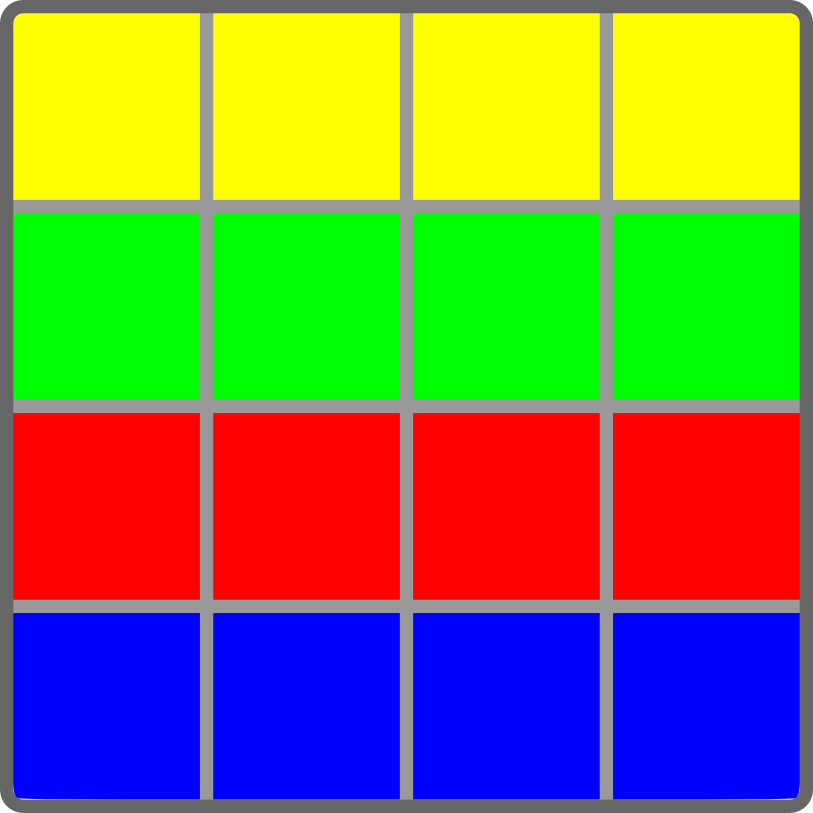
\includegraphics[width=0.55\textwidth]{images/rowPartitioning.png}
		\caption{Row partitioning}
		\label{fig:rowPartitioning}
	\end{subfigure}
	\begin{subfigure}{.3\linewidth}
		\centering
		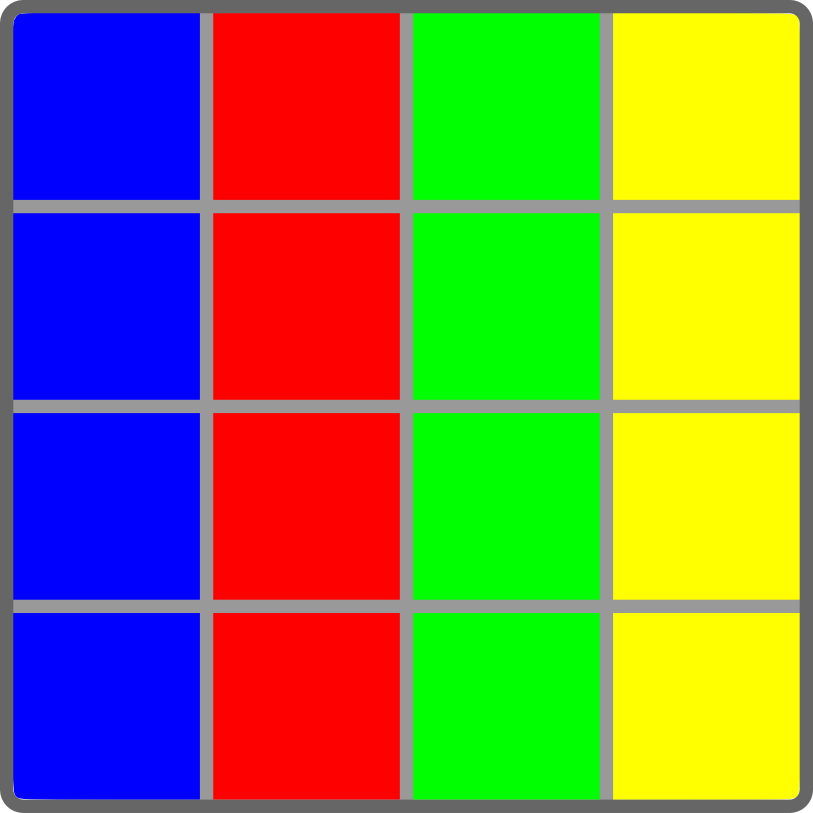
\includegraphics[width=0.55\textwidth]{images/columnPartitioning.png}
		\caption{Column partitioning}
		\label{fig:columnPartitioning}
	\end{subfigure}
	\begin{subfigure}{.3\linewidth}
		\centering
		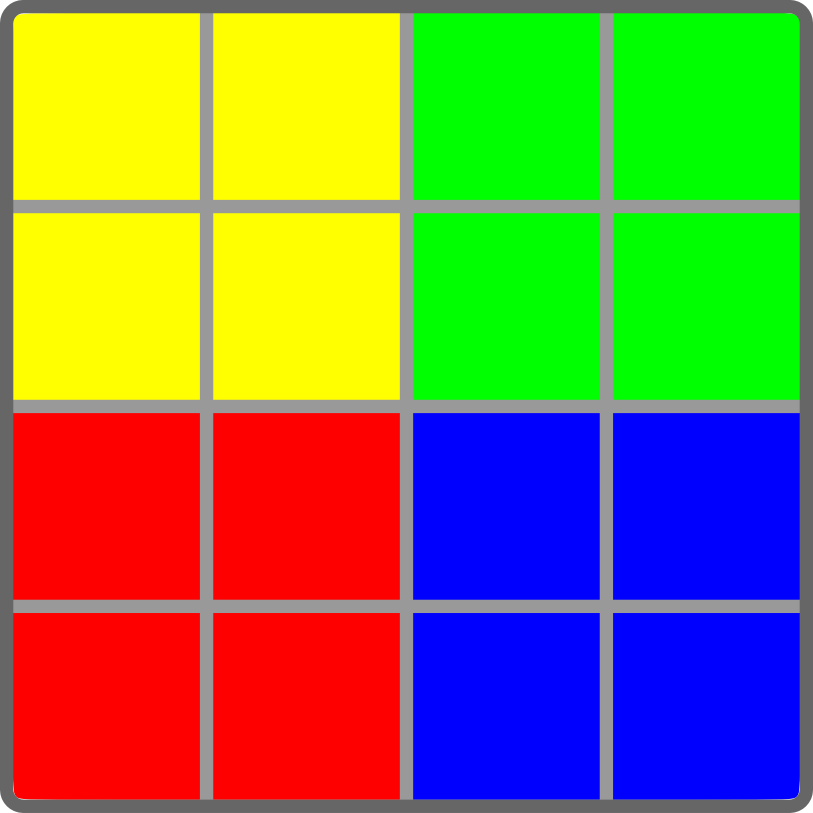
\includegraphics[width=0.55\textwidth]{images/quadraticBlockPartitioning.png}
		\caption{Square block partitioning}
		\label{fig:quadraticBlockPartitioning}
	\end{subfigure}
	\caption{Row-wise, column-wise and square block-wise matrix partitioning.}
	\label{fig:Partitionings}
\end{figure}

This approach, however, unveils its drawbacks when multiplying two equally partitioned matrices $A$ and $B$. 
In such a case, the row $r$ of $A$ and the complete matrix $B$ is needed to calculate the resulting row with index $r$. 
This circumstance implies a complete repartitioning of $B$. 
The repartitioning is especially grave, since $B$ has to be broadcasted to every row of $A$. 
In order to quantify the repartitioning costs of such a matrix multiplication, a simple cost model is developed. 
First of all, it is limited to modeling the communication costs, since network I/O usually constitutes the bottleneck of distributed systems. 
For the sake of simplicity, the multiplication of two quadratic matrices $A \in \mathbb{R}^{n\times n}$ and $B \in \mathbb{R}^{n\times n}$ giving the matrix $C\in \mathbb{R}^{n \times n}$ is considered. 
Moreover, we assume that there are $n$ worker nodes available, each of which receiving a single row of $A$ and $B$, respectively. 
Thus, $A$ and $B$ are row-wise partitioned. 
We further assume that rows with the same index are kept on the same worker node. 
Each row $a_r$ requires the complete knowledge of matrix $B$ in order to produce the row $c_r$. 
Therefore, every row $b_r$ has to be sent to all other worker nodes. 
Thus, the number of rows sent by each worker node is $n-1$. 
All of the $n$ worker nodes have to do the same. 
Consequently, the total number of sent messages is $n(n-1)$ and each message has a size of $n\alpha$ where $\alpha$ is the size of a matrix entry. 
Usually, each sending operation causes some constant overhead inflicted by resource allocation. 
Before sending the actual data over the network, memory to transfer the data to the network interface has to be allocated, network resources have to be reserved and a network connection with the remote peer has to be established. 
This overhead is denoted by $\Delta$. 
Since all sending operations occur in parallel, the costs caused by constant overhead are $(n-1)\Delta$. 
The total amount of data, which has to be sent over the network, is $n^2(n-1)\alpha$. 
The network interconnection is assumed to guarantee every node a bandwidth $\nu$. 
Therefore, the time needed for sending the data is $\frac{n^2(n-1)\alpha}{\nu}$. 
These considerations lead to the following repartitioning cost model:
\begin{displaymath}
	cost_{row} = \frac{n^2(n-1)\alpha}{\nu} + (n-1)\Delta
\end{displaymath}
Row and column partitioning are extreme forms of blocking. 
A less extreme form is to split the matrix into equally sized quadratic blocks as shown in \cref{fig:quadraticBlockPartitioning}. 
In order to identify the individual blocks, each of them will be a block row and block column index assigned. 
Thus, blocking adds some memory overhead in the form of index information. 
The blocks are distributed across the worker nodes. 
The block size directly controls the granularity of the partitioning. 
Increasing the block size will reduce the memory overhead of distributed matrices while reducing the degree of parallelism. 
Thus, the user has to adjust the block size value depending on the matrix sizes and the number of available worker nodes in order to obtain best performance. 
The quadratic block partitioning has similar properties like the row- and column-wise partitioning scheme when it comes to cellwise operations. 
We simply have to join corresponding blocks with respect to the pair of block row and column index and execute the operation on matching blocks locally. 
But how does this pattern performs for matrix multiplications? 
The assumptions are the same as before and additionally it is assumed that $n$ is a square number. 
Since the matrices $A$, $B$ and $C$ are equally partitioned into square blocks, indices will henceforth reference the block and not the matrix entry. In order to calculate the block $c_{ij}$, we have to know the block row $a_{i}$ and the block column $b_{j}$. 
The resulting block will be stored on the node $n_{ij}$ which already contains the blocks $a_{ij}$ and $b_{ij}$. 
Thus, each node $n_{ij}$ has to receive the missing $2\left(\sqrt{n}-1\right)$ blocks from the block row $a_{i}$ and block column $b_{j}$. 
In total, all worker nodes have to send $2n\left(\sqrt{n}-1\right)$ blocks. 
Each block has the size $n\alpha$. 
The total communication costs comprises the transmission costs and the network overhead:
\begin{displaymath}
	cost_{squareBlock} = \frac{2n^2\left(\sqrt{n}-1\right)\alpha}{\nu} + 2\left(\sqrt{n}-1\right)\Delta
\end{displaymath}
We see that the term $(n-1)$ is replaced by $2\left(\sqrt{n}-1\right)$ in the square block cost model. 
For $n>2$, the square block partitioning scheme is thus superior to the row- and column-wise partitioning pattern with respect to the cost model. 
The reason for this outcome is that the square blocks promote more localized computations compared to the other partitionings. 
Instead of having to know the complete matrix $B$, we only have to know one block row of $A$ and one block column of $B$ to compute the final result. 

Due to these advantages and its simplicity, we decide to implement the square block partitioning scheme in Gilbert. 
It would also be possible to combine different partitionings and select them dynamically based on the data sizes and input partitionings. 
Besides the partitioning, Gilbert also has to represent the individual matrix blocks. There exist several storing schemes for matrices depending on the sparsity of the matrix. 
For example, if a matrix is dense, meaning that it does not contain many zero elements, the elements are best stored in a continuous array. 
If a matrix is sparse, then a compressed representation is best suited. 
Gilbert chooses the representation of each block dynamically. 
Depending on the non-zero elements to total elements ratio, a sparse or dense representation is selected.

\subsection{Linear Algebra Operations}
\label{sec:LinearAlgebraOperations}

In the following, we will outline the implementation of the matrix multiplication operator, which is most critical for performance in linear algebra programs. 
For a reference of the implementation of the remaining operators, we refer the interested reader to~\cite{Rohrmann2014}. 
Note that we use the Breeze~\cite{breeze} library for conducting local linear algebraic operations. 
In a MapReduce-like system there exist two distinct matrix multiplication implementations for square blocking. 
The first approach is based on replicating rows and columns of the operands and is called replication based matrix multiplication (RMM). 
The other method is derived from the outer product formulation of matrix multiplications. 
It is called cross product based matrix multiplication (CPMM). 

Let us assume that we want to calculate $A \times B = C$ with $A,B$ and $C$ being matrices. 
The block size has been chosen such that $A$ is partitioned into $m\times l$ blocks, $B$ is partitioned into $l \times n$ blocks and the result matrix $C$ will be partitioned into $m\times n$ blocks. 
In order to reference the block in the $i$th block row and $j$th block column of $A$, we will write $A_{ij}$. 
A block row will be denoted by a single subscript index and a block column by a single superscript index. 
For example, $A_i$ marks the $i$th block row of $A$ and $A^j$ the $j$th block column of $A$. 
The replication-based strategy will copy for each $C_{ij}$ the $i$th block row of $A$ and the $j$th block column of $B$. 
The replicated blocks of $A_i$ and $B^j$ will be grouped together. 
These steps can be achieved by a single mapper. 
Once this grouping is done, the final result $C_{ij}$ can be calculated with a single reducer. 
The reduce function simply has to calculate the scalar product of $A_i$ and $B^j$. 
It is important to stress that $A_i$ is replicated for each $C_{ik},\forall k$. 
The whole process is illustrated in \cref{fig:RMM}.

\begin{figure}[h!]
	\centering
	\begin{subfigure}{.43\linewidth}
		\centering
		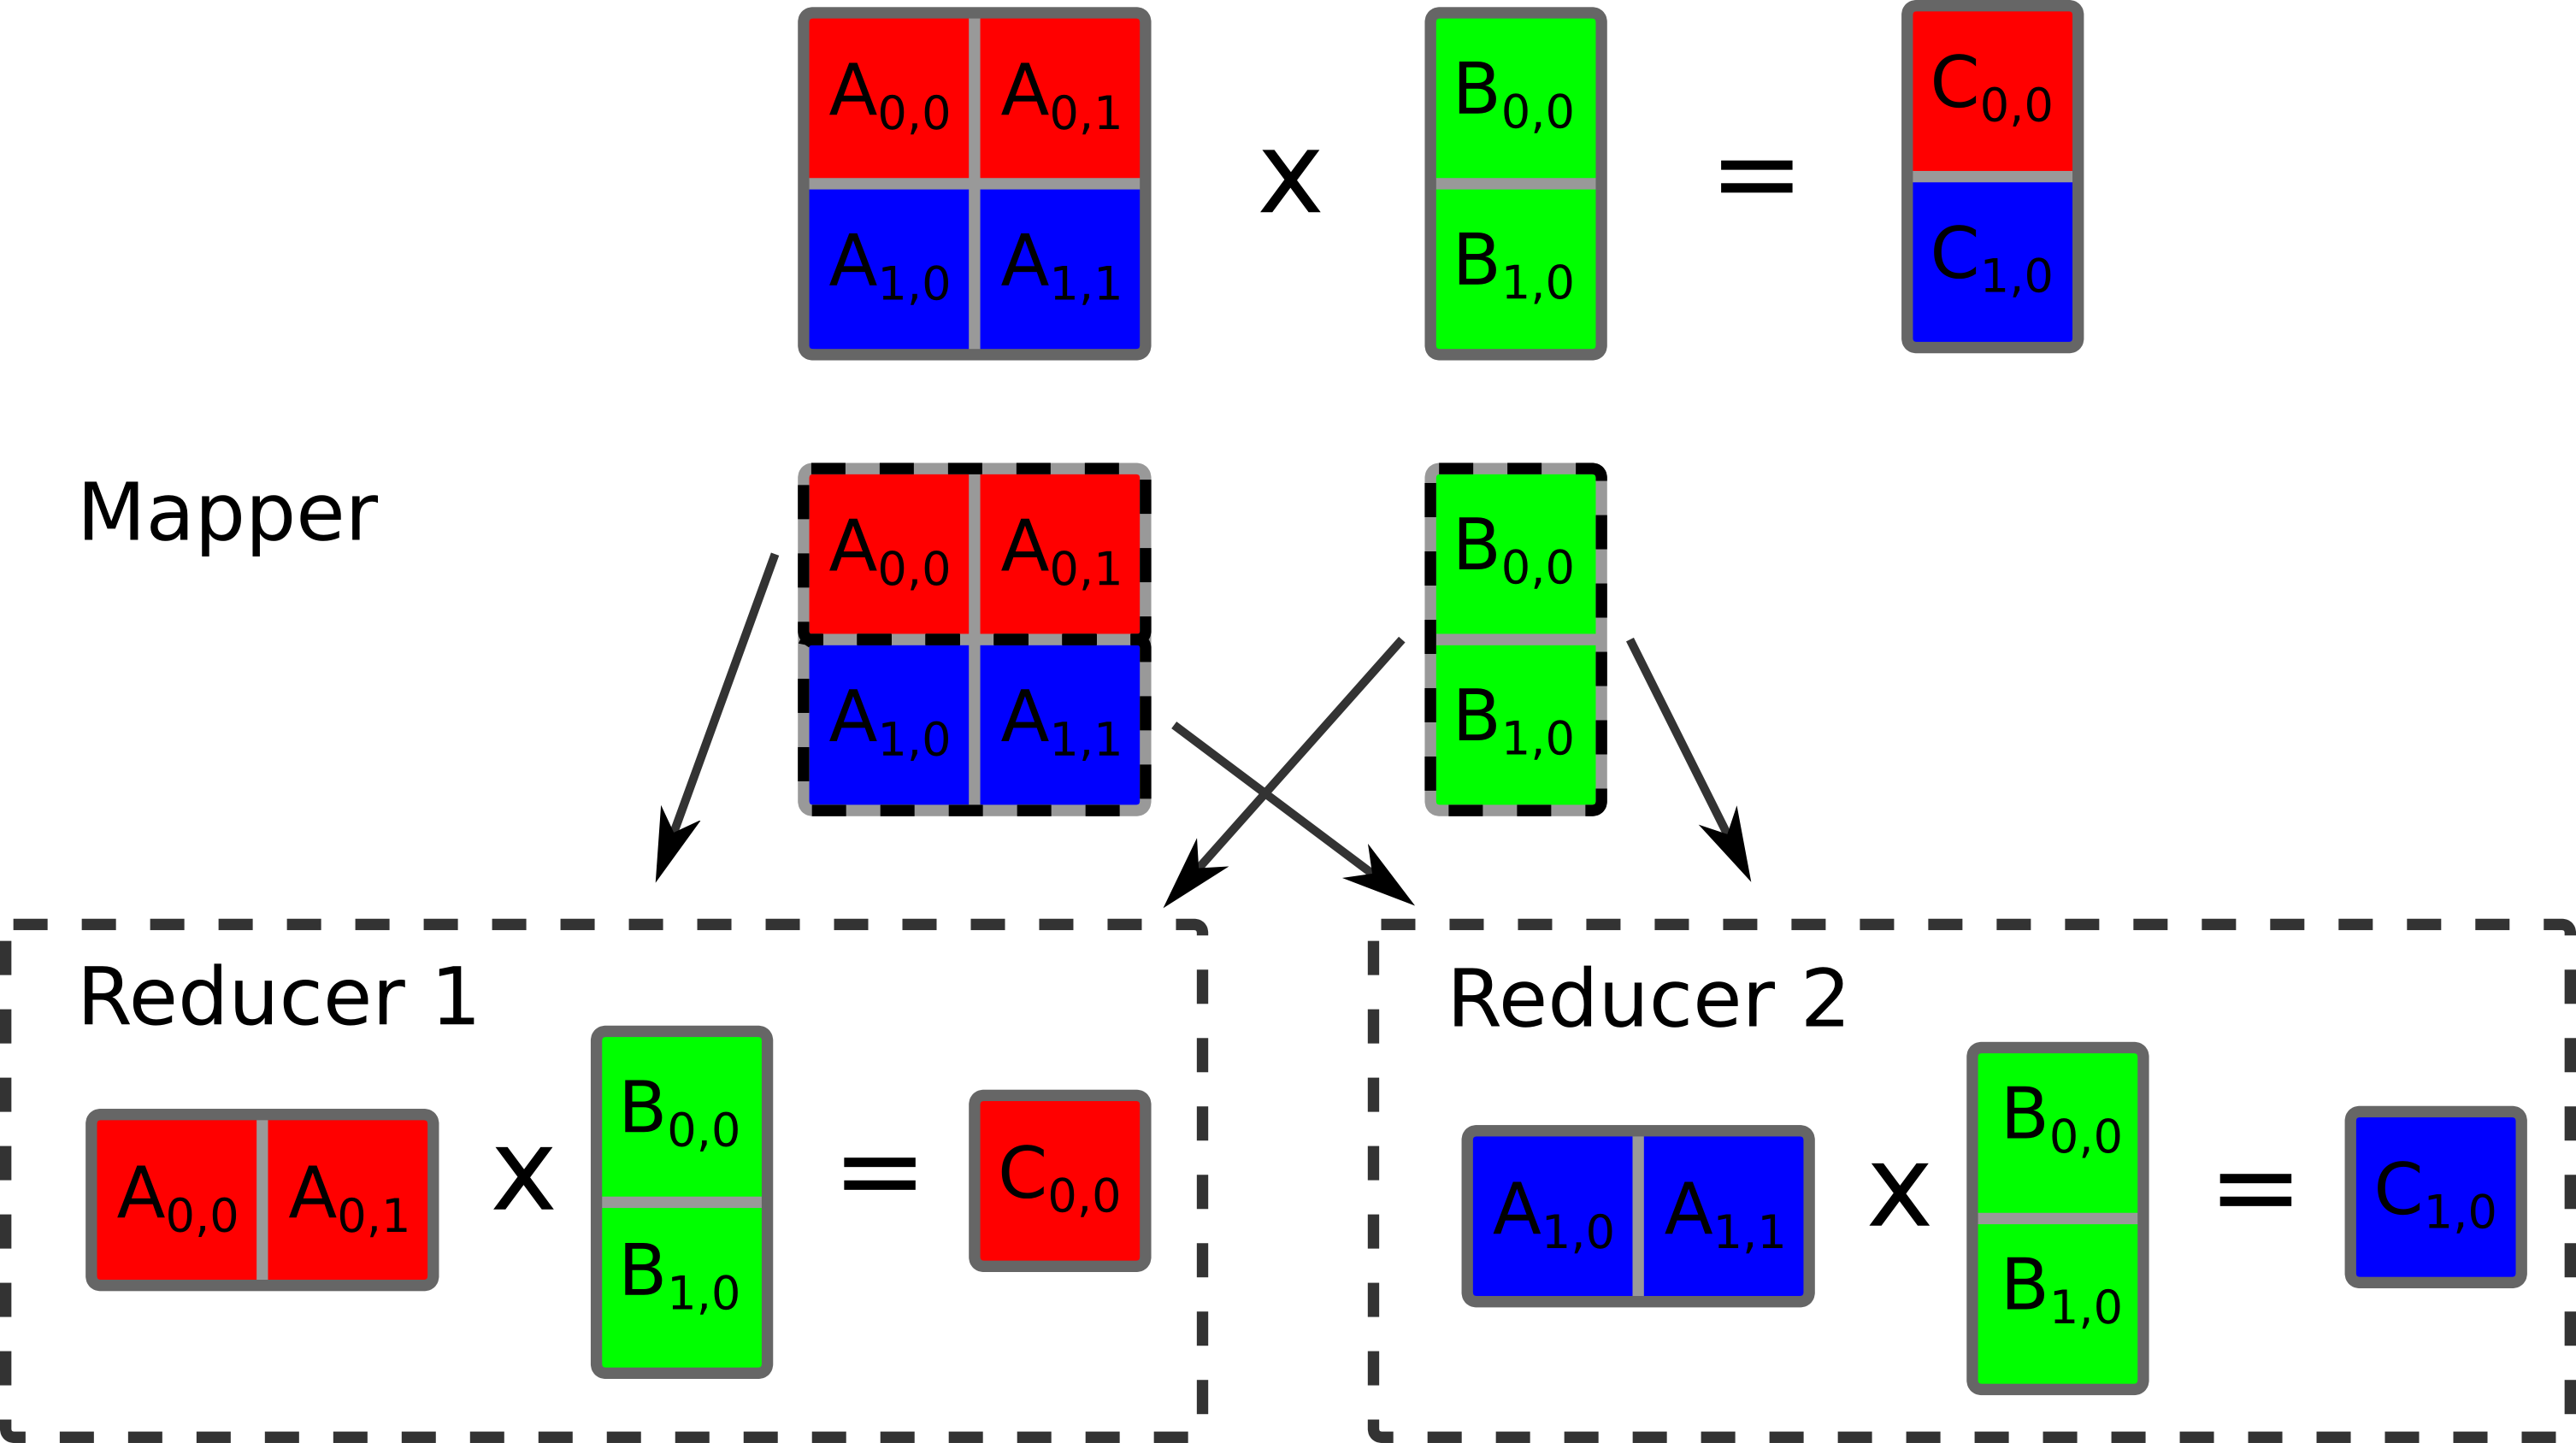
\includegraphics[width=0.99\linewidth]{images/rmm.png}
		\caption{Replication based matrix multiplication.}
		\label{fig:RMM}
	\end{subfigure}
	\hfill
	\begin{subfigure}{.43\linewidth}
		\centering
		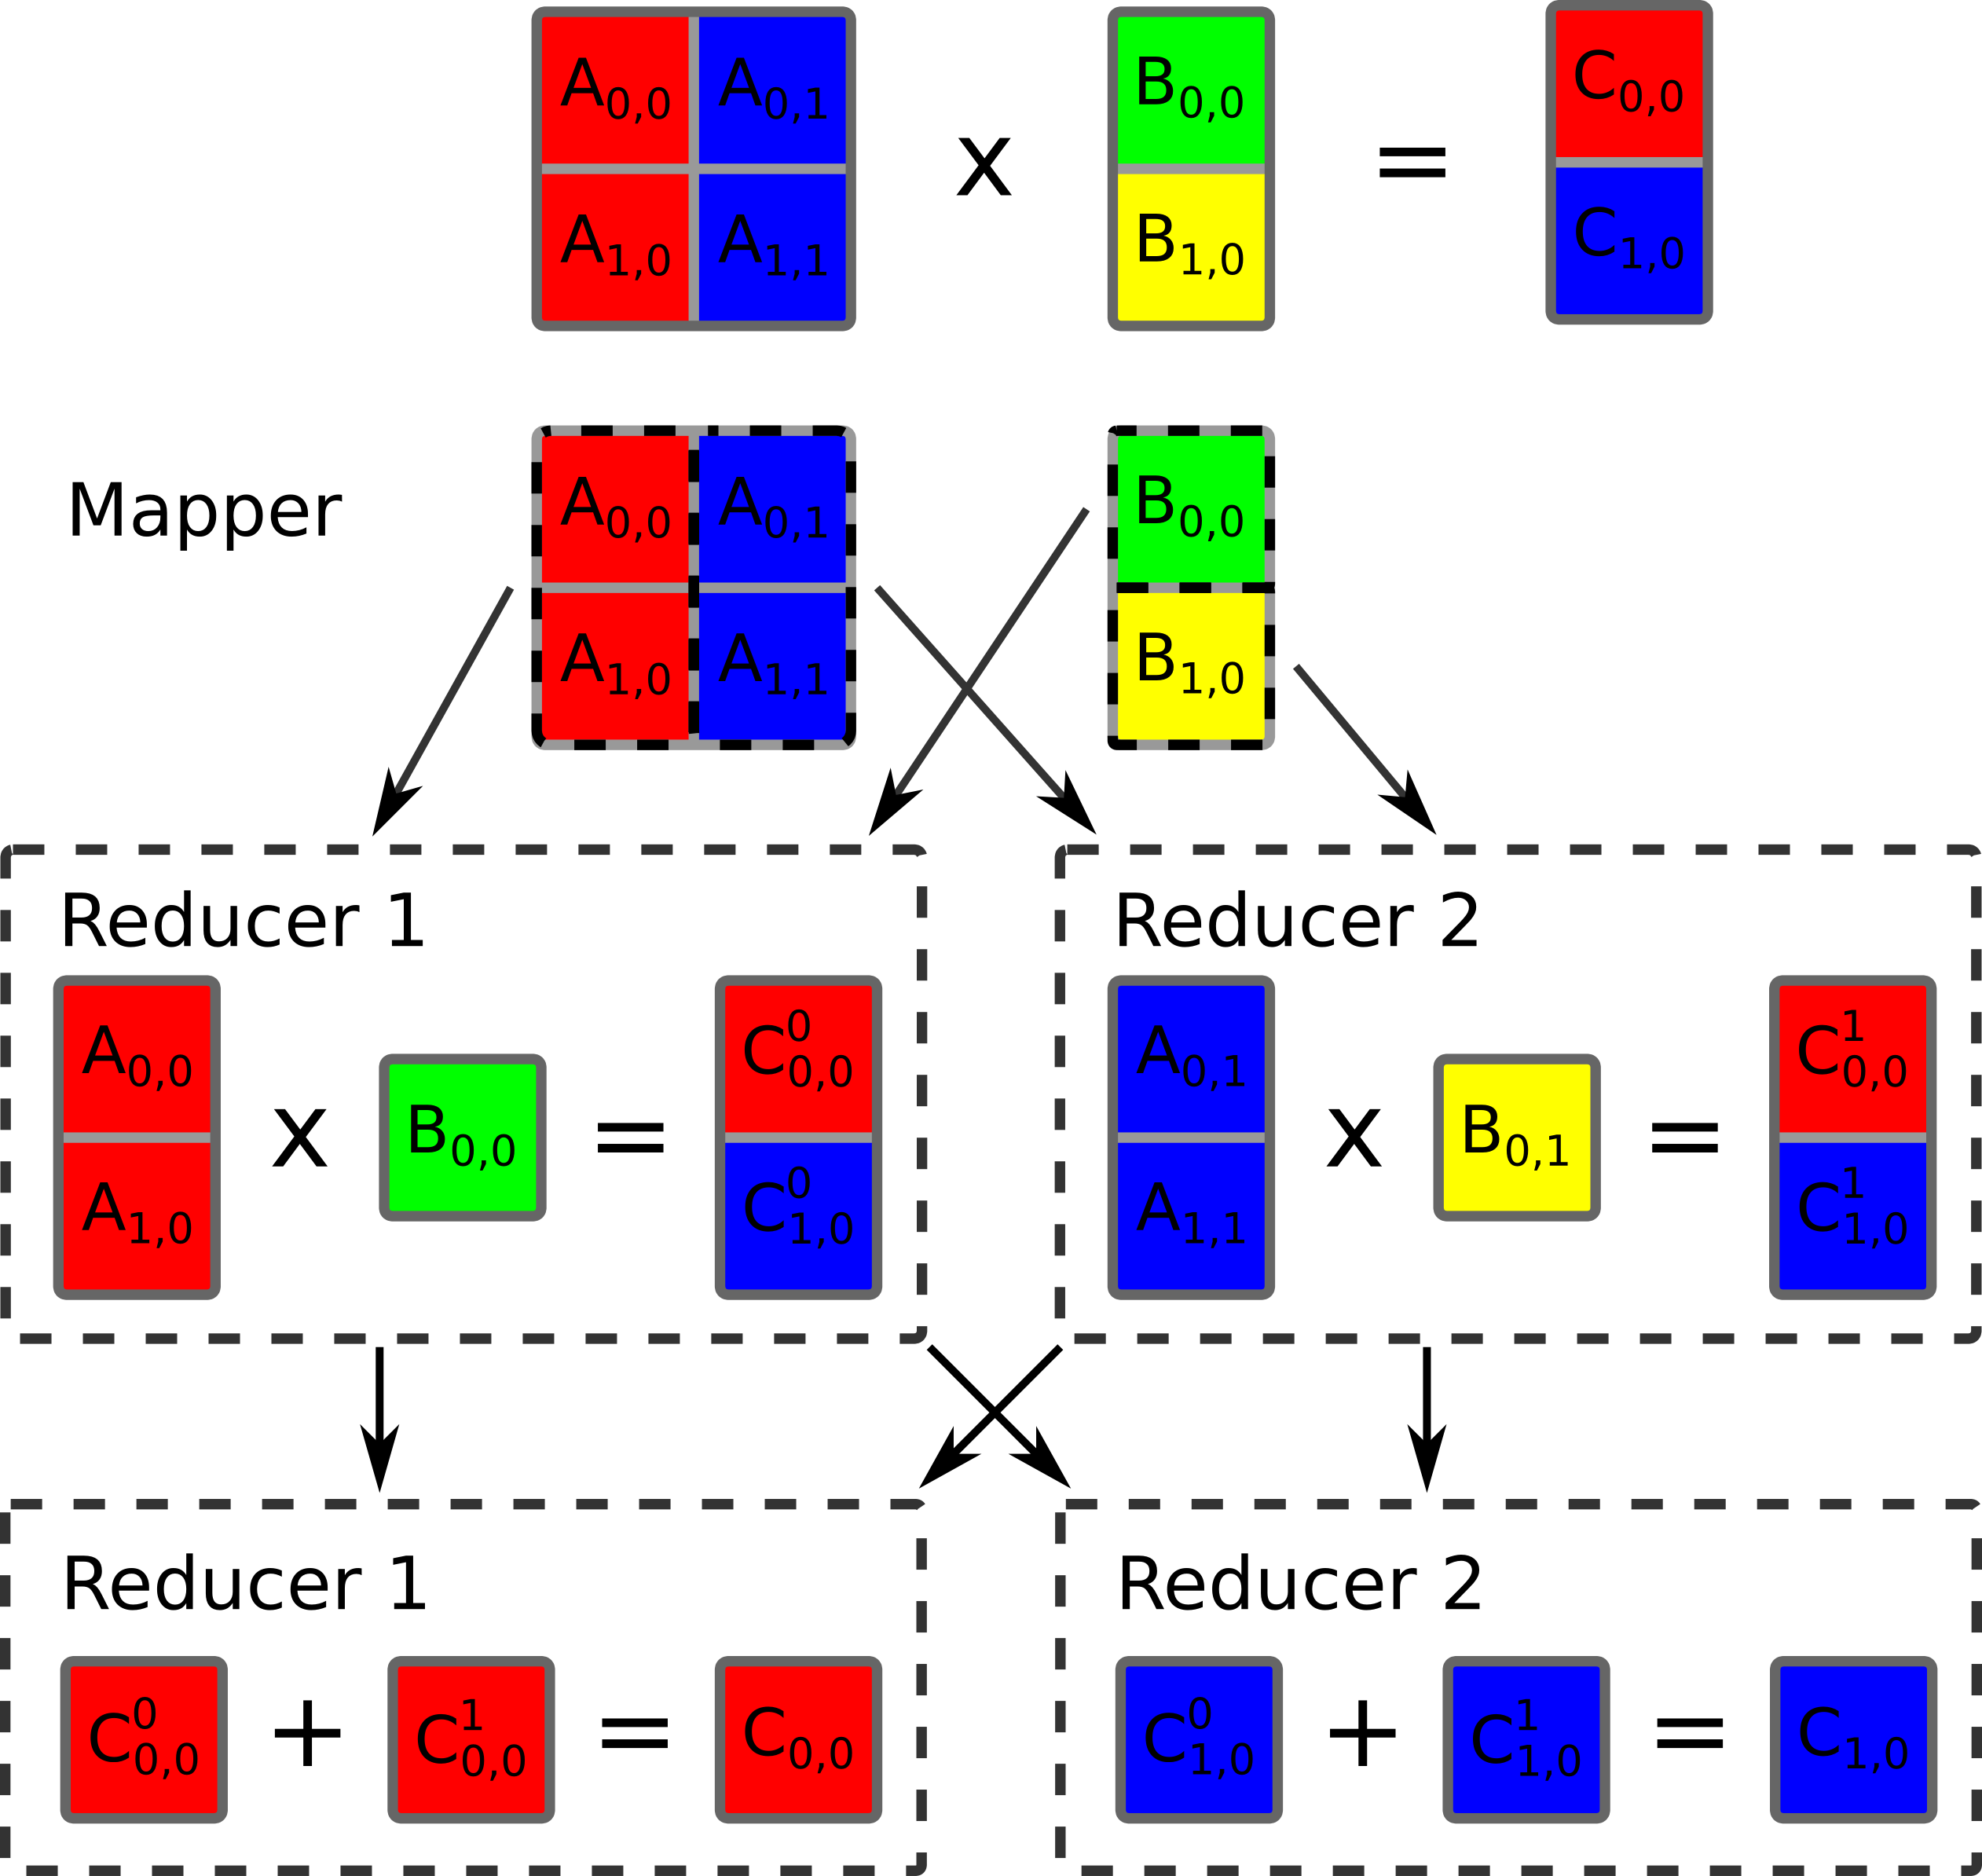
\includegraphics[width=0.8\linewidth]{images/cpmm.png}
		\caption{Cross product matrix multiplication.}
		\label{fig:CPMM}
	\end{subfigure}
	\caption{Execution strategies for matrix multiplication in MapReduce.}
	\label{fig:MMs}
\end{figure}

In contrast to RMM, CPMM calculates the outer products between $A^k$ and $B_k$ for all $k$. 
A mapper can group the $A^k$ and $B_k$ together so that a reducer can compute the outer products. 
Consequently, this method does not replicate any data. 
The outer product produces intermediate result matrices $C^k$ which have to be added up to produce the final result $C=\sum_{k=1}^{l} C^k$. 
This summation can be achieved by a subsequent reducer. 
The whole process is illustrated in \cref{fig:CPMM}. 

The methods RMM and CPMM differ in terms of network communication. 
The former method can be realized within a single MapReduce job whereas the latter requires two. 
Neither RMM nor CPMM is always superior. 
The optimal matrix multiplication strategy depends on the matrix size of its operands $A$ and $B$. 
Fortunately, Flink and Spark exhibit a little bit more flexibility in terms of higher order functions. 
Looking at the definition of the matrix multiplication for $C_{ij}=\sum_{k=1}^{l}A_{ik}\times B_{kj}$, it can be seen that every $A_{ik}$ has to be joined with its corresponding $B_{kj},\forall k$. 
This pairwise mapping can be easily achieved by using the join function. 
The join-key is the column index of $A$ and the row index of $B$. 
The joiner calculates for each matching pair $A_{ik}$ and $B_{kj}$ an intermediate result $C_{ij}^k$. 
Grouping the intermediate results with respect to the index pair $(i,j)$ allows us to compute the final result in a subsequent reduce step. 
The overall algorithm strongly resembles the CPMM. 

Flink supports several execution strategies for the higher-order functions. 
A cost-based optimizer selects the best strategies prior to execution. 
One possible optimization concerns the join function. 
The join can either be realized using a broadcast hash join, a repartitioning hash join or a repartitioning sort-merge join algorithm depending on the current partitioning and the input data sizes. 
If one input data is relatively small compared to the other input, it is usually more efficient to use the broadcast hash join algorithm. 

Without loss of generality, we assume that the matrix $B$ constitutes such a small input. 
If we further assume that the block rows of $A$ are kept on the same worker node, then the last reduce operation can be executed locally and without any shuffling. 
The resulting execution plan under these assumptions is equivalent to the RMM. 
If the system chooses any of the repartitioning join algorithms instead, then the columns of $A$ will be distributed across the worker nodes. 
Consequently, the last reduce step causes a mandatory repartitioning. 
Then, the resulting execution plan is equivalent to the CPMM. 
Even though Gilbert has only one dataflow plan specified to implement the matrix multiplication, the Flink system can choose internally between the RMM and CPMM strategy. 
The strategy is selected by the optimizer which bases its decision on the data size and the partitioning, if available.